% =============================================================================
\section{Results}\label{sec:results}
% =============================================================================
The completed result table contains one real baseline and 480 complex configurations. All values in this section are regenerated from the supplied experiment CSV. Because the same fixed patient test cohort is used for the entire architecture grid, the factor-level and top-configuration summaries are descriptive.

\subsection{Overall Factorial Performance}
The real magnitude baseline achieved test AUC \RealAUC and AP \RealAP. Across the 480 complex configurations, AUC ranged from \ComplexMinAUC to \BestAUC, with mean AUC \ComplexMeanAUC and mean AP \ComplexMeanAP. \ComplexWins/\ComplexTotal complex configurations exceeded the real-baseline AUC.

\begin{figure}[!t]
\centering
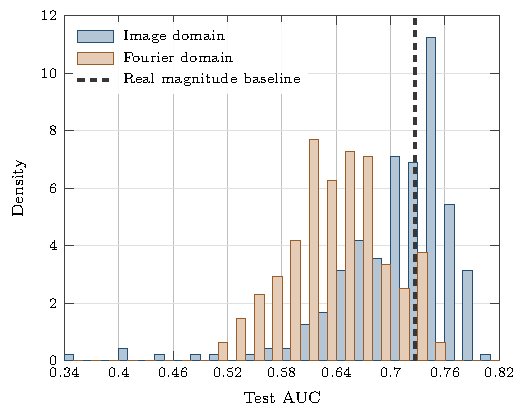
\includegraphics[width=\columnwidth]{../figures/results_auc_landscape/figure_auc_landscape_artwork.pdf}
\caption{Distribution of test AUC across the 480 complex-valued configurations. Image-domain and Fourier-domain configurations are shown using identical histogram bins; the dashed vertical line denotes the fixed real magnitude baseline.}
\label{fig:auc-landscape}
\end{figure}

\subsection{Input-Domain Summary}
The real magnitude baseline achieved test AUC $0.7268$. The complex grid contains 480 configurations, split evenly between 240 image-domain and 240 Fourier-domain configurations. Image-domain complex models had mean AUC $0.7102$ and Fourier-domain complex models had mean AUC $0.6377$, giving the broadest observed separation between the two input domains. The matched domain comparison covers 240 architecture pairs; image-domain AUC exceeded Fourier-domain AUC in 196/240 pairs ($81.7\%$), with mean paired $\Delta$AUC (image minus Fourier) $+0.0725$ and median paired $\Delta$AUC $+0.0852$. These paired quantities, together with the Wilcoxon signed-rank statistic and rank-biserial effect size in the table, are descriptive properties of the finite factorial grid and are not interpreted as population-level inference.

\begingroup
\renewenvironment{table}{\begin{table*}}{\end{table*}}
% Requires: \usepackage{booktabs}

\begin{table}[t]
\centering
\small
\setlength{\tabcolsep}{3pt}
\caption{Descriptive summary of test AUC for the observed image-domain and Fourier-domain complex configurations. Percentages count configurations exceeding the fixed real magnitude baseline (AUC $=0.7268$).}
\label{tab:results_auc_landscape_summary}
\begin{tabular}{lrrrrrrrr}
\toprule
Domain & $n$ & Mean & SD & Median & IQR & Min & Max & $>$ baseline, $n$ (\%) \\
\midrule
Image   & 240 & 0.7102 & 0.0665 & 0.7251 & 0.0740 & 0.3464 & 0.8162 & 116 (48.3) \\
Fourier & 240 & 0.6377 & 0.0536 & 0.6384 & 0.0689 & 0.5037 & 0.7534 & 14  (5.8) \\
\bottomrule
\end{tabular}
\end{table}

\begin{table}[t]
\centering
\small
\setlength{\tabcolsep}{5pt}
\caption{Paired descriptive comparison of test AUC for matched image-domain and Fourier-domain configurations. Each pair holds pooling, normalization, convolution, activation, stream level, and interaction level fixed. The Wilcoxon signed-rank result and paired rank-biserial effect size are descriptive measures for the observed factorial pairs, not strong population inference.}
\label{tab:results_auc_landscape_separation}
\begin{tabular}{lr}
\toprule
Measure & Value \\
\midrule
Number of matched pairs & $240$ \\
Mean paired $\Delta$AUC (image $-$ Fourier) & $+0.0725$ \\
SD of paired $\Delta$AUC & $0.0877$ \\
Median paired $\Delta$AUC & $+0.0852$ \\
IQR of paired $\Delta$AUC & $0.1125$ \\
$\Delta$AUC $>0$, $n$ (\%) & $196$ (81.7) \\
Wilcoxon signed-rank statistic & $3471.5$ \\
Wilcoxon $p$-value (two-sided) & $1.86\times10^{-24}$ \\
Paired rank-biserial effect size & $+0.7599$ \\
\bottomrule
\end{tabular}
\end{table}

\endgroup

\subsection{Factor-Level Summaries and Selected Interactions}
The marginal factor table reports descriptive means across the finite complex grid; its $\Delta$ column is mean AUC at that factor level minus the overall complex-grid mean AUC. Normalization shows a visible marginal contrast, with complex BatchNorm higher than RMSNorm, whereas convolution and activation contrasts are comparatively smaller. The interaction table retains the implemented five-level combined stream/interaction factor (complex-only/none, complex-only/holographic, dual/none, dual/modulus gate, and dual/holographic) rather than treating stream and interaction as separate independent factors. The stream/interaction pattern depends on domain, while the image/Fourier domain contrast remains the largest broad marginal separation. These summaries are descriptive properties of the observed factorial grid and do not establish a universal operator ranking.

\begingroup
\renewenvironment{table}{\begin{table*}}{\end{table*}}
% Requires \usepackage{booktabs}.
\begin{table}[t]
\centering
\caption{Descriptive marginal factor-level summaries of test AUC over the 480 complex configurations. $\Delta$ denotes mean AUC minus the overall complex-grid mean.}
\label{tab:factor-effects-marginal}
\small
\begin{tabular}{llrrrrrr}
\toprule
Factor & Level & $n$ & Mean AUC & SD & Median & IQR & $\Delta$ \\
\midrule
Pooling & max & 160 & 0.671 & 0.077 & 0.674 & 0.096 & -0.003 \\
 & median & 160 & 0.673 & 0.070 & 0.673 & 0.110 & -0.001 \\
 & average & 160 & 0.678 & 0.063 & 0.679 & 0.099 & 0.004 \\
Normalization & RMSNorm & 240 & 0.663 & 0.076 & 0.666 & 0.113 & -0.011 \\
 & C-BatchNorm & 240 & 0.685 & 0.063 & 0.684 & 0.093 & 0.011 \\
Convolution & standard & 240 & 0.677 & 0.069 & 0.678 & 0.104 & 0.003 \\
 & widely linear & 240 & 0.671 & 0.072 & 0.673 & 0.109 & -0.003 \\
Activation & modReLU & 120 & 0.680 & 0.061 & 0.684 & 0.092 & 0.006 \\
 & Mag-SiLU & 120 & 0.671 & 0.069 & 0.666 & 0.111 & -0.003 \\
 & CReLU & 120 & 0.673 & 0.075 & 0.676 & 0.111 & -0.001 \\
 & cardioid & 120 & 0.671 & 0.076 & 0.673 & 0.103 & -0.003 \\
Stream/interaction & C-only / none & 96 & 0.672 & 0.068 & 0.676 & 0.087 & -0.002 \\
 & C-only / holo & 96 & 0.652 & 0.076 & 0.664 & 0.081 & -0.022 \\
 & Dual / none & 96 & 0.679 & 0.074 & 0.678 & 0.133 & 0.005 \\
 & Dual / gate & 96 & 0.690 & 0.058 & 0.703 & 0.086 & 0.016 \\
 & Dual / holo & 96 & 0.677 & 0.070 & 0.685 & 0.120 & 0.003 \\
\bottomrule
\end{tabular}
\end{table}

% Requires \usepackage{booktabs}.
\begin{table}[t]
\centering
\caption{Descriptive domain-by-factor interaction summaries of test AUC. Each cell averages over the remaining factorial dimensions.}
\label{tab:factor-effects-interactions}
\small
\begin{tabular}{llrrrrr}
\toprule
Domain & Level & $n$ & Mean AUC & SD & Median & IQR \\
\midrule
\multicolumn{7}{l}{\textit{Domain $\times$ normalization}} \\
Image & RMSNorm & 120 & 0.695 & 0.079 & 0.714 & 0.086 \\
 & C-BatchNorm & 120 & 0.725 & 0.046 & 0.734 & 0.056 \\
Fourier & RMSNorm & 120 & 0.631 & 0.056 & 0.623 & 0.075 \\
 & C-BatchNorm & 120 & 0.645 & 0.050 & 0.648 & 0.058 \\
\midrule
\multicolumn{7}{l}{\textit{Domain $\times$ stream/interaction}} \\
Image & C-only / none & 48 & 0.682 & 0.079 & 0.690 & 0.093 \\
 & C-only / holo & 48 & 0.670 & 0.087 & 0.681 & 0.060 \\
 & Dual / none & 48 & 0.741 & 0.033 & 0.748 & 0.032 \\
 & Dual / gate & 48 & 0.725 & 0.044 & 0.732 & 0.048 \\
 & Dual / holo & 48 & 0.734 & 0.039 & 0.740 & 0.050 \\
Fourier & C-only / none & 48 & 0.662 & 0.055 & 0.660 & 0.082 \\
 & C-only / holo & 48 & 0.634 & 0.059 & 0.638 & 0.067 \\
 & Dual / none & 48 & 0.617 & 0.045 & 0.615 & 0.070 \\
 & Dual / gate & 48 & 0.656 & 0.050 & 0.656 & 0.077 \\
 & Dual / holo & 48 & 0.620 & 0.044 & 0.619 & 0.053 \\
\bottomrule
\end{tabular}
\end{table}

\endgroup

\subsection{Canonical Pooling Ablation}
The canonical comparison fixes image-domain input, ComplexRMSNorm2d (RMSNorm), standard complex convolution, a complex-only stream, no interaction, and modReLU. The three complex configurations differ only in the complex pooling operator: canonical max-pool, canonical median-pool, and canonical average-pool. Table~\ref{tab:canonical-comparison} reports these configurations together with the fixed real magnitude baseline for direct comparison.

\begingroup
\renewenvironment{table}{\begin{table*}}{\end{table*}}
\input{../tables/canonical_comparison/canonical_comparison.tex}
\endgroup

\subsection{High-Performing Configurations}
The maximum observed factorial AUC was \BestAUC with AP \BestAP for configuration \texttt{\BestLabel}. This is an exploratory maximum over the fixed 480-configuration grid evaluated on the same held-out test cohort, not an unbiased estimate of a selected final architecture.

\subsection{Joint AUC--AP Landscape}

Across the finite 480-configuration factorial grid, 114/480 complex configurations (23.8\%) exceeded the real baseline in both AUC and AP. This occurred for 101/240 image-domain configurations (42.1\%) and 13/240 Fourier-domain configurations (5.4\%). Across all configurations, AUC and AP showed a Pearson correlation of $r=0.755$ and a Spearman rank correlation of $\rho=0.788$. These quadrant counts and correlations are descriptive properties of the observed finite factorial grid.
